In this section, we describe the different provisioning techniques implemented in ConPaaS.



\subsection{Load-based provisioning}


The existing infrastructures offer provisioning mechanisms that adjust the amount of resources based on the load of the currently allocated resources. Within this group of provisioning mechanisms, we include the simple trigger-based systems that define threshold rules to increase and decrease the computational power of an application in order to guarantee several performance requirements. As an example, the Auto Scaling system offered by Amazon EC2~\cite{amazonEC2} scales out an application whenever its CPU usage in the last 10min exceeds a specific threshold (Amazon recommends to establish an upper bound of 70\%).  This rules-based technique is currently used in mature cloud platforms such as RightScale~\cite{right-scale} or OpenShift~\cite{openshift}. 

For the sake of comparison, we decided to design and implement a trigger-based provisioning mechanism in ConPaaS, called "load-based provisioning". This algorithm monitors CPU usage and response time metrics, and dynamically adjusts the computational power of an application by analyzing whether the monitoring data exceed their thresholds~\footnote{Every metric has a threshold range (max,min).}, as illustrated in Algorithm~\ref{loadBased_prov}. Obviously, the lower and upper bound of each threshold are pre-defined by the user before execution.

\begin{algorithm}
{\scriptsize
\SetAlgoLined
\SetInd{0mm}{2mm}
\KwData{\\
\hspace{3mm} System-level metrics (CPU, Resp. time)\\
\hspace{6mm} - Pre-defined metric threshold ranges, \emph{thr}
}
\KwResult{Scaling decisions}
\BlankLine
\While{auto-scaling is ON}{
Collect monitoring data of each metric, \emph{data}\;
\BlankLine
\While{ no recent scaling operation}{
\uIf{ avg(data$_i$) $>=$ \emph{thr}$_i$  }{
ADD resources\;
}
\ElseIf{ avg(data$_i$) $<$ \emph{thr}$_i$  }{
REMOVE resources\;
} 
}
}
}
\caption{Load-based}
\label{loadBased_prov}
\end{algorithm}

% , expressed in the form of a Service Level Agreement

\subsubsection{Problematic of this algorithm}

Even though these type of mechanisms are simple and widely used in cloud platforms, they are excessively reactive and not so precise when provisioning web applications due to several factors: 

%regarding the decision making process

\begin{itemize}
\item  \textbf{Workload mix and web traffic:} In web applications, the system performance behavior fluctuates following an irregular pattern caused by the traffic and its workload mix, which increase the complexity to predict future fluctuations. 

%Obviously, a reactive algorithm can be seen a good choice for resource provisioning, however. The system %performance of an application change in time if the type of workload changes.

\item \textbf{Reactiveness:} An excessively reactive system can affect the system performance when handling flash crowds or slashdot effects. A high frequency of scaling operations can provokes sharp and sudden fluctuations that affect the performance instead of improving it, as well as increases the infrastructure cost. So, it is particularly difficult to decide when to scale out or back an application. 

\item \textbf{Services as black boxes:} Services are handled as black boxes, the definition of threshold rules often only covers system-level metrics such as response time and CPU usage. Therefore, when provisioning web applications, metrics such as request rate of static/dynamic files may be also taken into consideration to improve the accuracy of the decisions.

% when handling web traffic.

%These constraints are too generic, as other application-specific constraints are not considered. 

%\item VMs are heterogeneous in performance, and thereby their throughput vary depending of its hardware configuration (instance's types). 
\item  \textbf{Heterogeneity:} The performance of virtual instances provided by current clouds is largely heterogeneous, even when requesting the exact same type of instance each time, as stated in~\cite{ec2Performance}. 

% The provisioning mechanism omit the heterogeneity of the VMs associated to host an application. 

\end{itemize}

Based on these factors, we believe trigger-based provisioning mechanisms can be optimized without drastically increasing its complexity. A solution seems to be the utilization of techniques that handle web traffic and workload mix without being excessively reactive. Moreover, the implementation of these techniques have to remain a simple exercise to facilitate its integration in existing auto-scaling systems. In the following we present two techniques that aims at solving the aforementioned drawbacks by relying on predictive and more accurate methods.

% to dynamically adjust the computational power to irregular workload pattern of web applications.


%previous knowledge about behavior of the application, avoid flash crowds too reactive
%and the definition of application-specific constraints 
%Tthe definition of threshold range based on how much workload a server can handle. what is the request %rate that a server can sustain without becoming overloaded?
%what is the value of the CPU utilization/load that indicates that a server is
%overloaded? These values are different from one application to another, and also
%from one server to another. 


%Second experiment: improved the basic provisioning with some application knowledge
%observed empirically (the maximum request rate we can send to a server, maybe also
%the maximum CPU utilization we can allow). The results show more stability in the
%provisioning.  


\subsection{Weighted-metric feedback provisioning}
Based on our previous knowledge from load-based provisioning, we designed and implemented an algorithm which improves the accuracy of our scaling actions when hosting web applications. To achieve that, our algorithm relies on three simple mechanisms: the definition of weights to each metric included in the performance requirements, the use of flexible thresholds and the estimation of the workload trend. 

%In order to handle temporal bursty workload, we designed and implemented a predictive and reactive algorithm by relying on
\vspace{2mm}

\textbf{Weighted metrics:} Traditional algorithms would scale out and back whenever a system-level metric exceeds its beforehand defined threshold range. Nevertheless,  through the definition of weight values to application and system metrics, our algorithm takes into consideration its weight when making scaling decisions. More precisely, when hosting web applications, our algorithm associates weights in an ascending order to the following metrics: request rate, CPU usage and response time. Accordingly the response time has a higher weight than the request rate, since higher values in the response time rapidly indicate the existence of a performance degradation in a web application. As detailed in Section~\ref{wikipedia}, scaling decisions only make based on the request rate can incur errors by under- or over-provisioning  a web application, due to the large diversity in the complexity of the requests~\cite{singh_autonomic_2010}.

%High values in the request rate cannot always indicate that an application is becoming overloaded, due to the large diversity in the complexity of the requests.


\begin{algorithm}
{\scriptsize
\SetAlgoLined
\SetInd{0mm}{2mm}
\KwData{\\
\hspace{3mm} System and App-level metrics\\
\hspace{6mm} - Pre-defined metric threshold ranges, \emph{threshold}\\
\hspace{3mm} Define the weight of each metric, \emph{w}
}
\KwResult{Scaling decisions}
\BlankLine
Create a queue to store historical workload, \emph{q}\;
Establish flexible thresholds from \emph{threshold} ranges\;
\hspace{3mm}	- Scalings operations could be triggered, \emph{pred\_thr}\;
\hspace{3mm}	- Scalings operations must be triggered, \emph{reac\_thr}\; 
\BlankLine
\While{auto-scaling is ON}{
Collect monitoring data of each metric, \emph{data}\;

\uIf{ avg(data$_i$) $>=$ pred\_thr$_i$}{
	Increment chances of \emph{scaling\_out} using \emph{w$_i$}, \emph{s\_out}\;
}\ElseIf{ avg(data$_i$) $<$ pred\_thr$_i$}{
	Increment chances of \emph{scaling\_in} using $w_i$, \emph{s\_in}\;
}
\BlankLine
Add to \emph{q} the most recent workload value\;
Estimate historical workload trends (last $\sim$30min), \emph{td}\;
\hspace{3mm}	- If trend is increasing then \emph{td} = 1\;
\hspace{3mm}	- If trend is decreasing then \emph{td} = 0\;	
\hspace{3mm}	- Undetermined \emph{td} = -1\;	
\BlankLine
\While{ no recent scaling operation}{
\uIf{ avg(data$_i$) $>=$ reac\_thr$_i$ \textbf{and}  $td$ = 1 \textbf{and} \emph{s\_out} $>$ \emph{s\_in}}{
	ADD resources\;
}
\ElseIf{ avg(data$_i$) $<$ reac\_thr$_i$ \textbf{and} \emph{td} = 0 \textbf{and} s\_out $<$ s\_in }{
	REMOVE resources\;
}
}
}
}
\caption{Weighted-metric feedback}
\label{history_prov}
\end{algorithm}


\textbf{Flexible thresholds:} This algorithm uses two levels of threshold ranges for each metric: \emph{predictive} and \emph{reactive}. As shown on Figure~\ref{flexibleThresholds}, there are two "head rooms" between the SLO (Service Level Objective) threshold (performance requirements pre-defined by the user) and the flexible thresholds.  First, the head-room $H_1$ is between the predictive threshold and the reactive thresholds, and is intended to alert of possible workload alterations in advance.  Thereby, when the system performance exceeds the predictive ranges, there is an increment in the chances of scaling actions will be triggered to tackle future SLO violations. The second head-room $H_2$ comprises between the SLO and reactive thresholds is used to trigger scaling actions. Performance values exceeding the reactive threshold launch scaling operations if other conditions are also satisfied. As an example of flexible thresholds for the CPU-usage, we established a predictive range comprised between 30\% and 70\% , and a reactive comprised between 20\% and 80\%.  

\begin{figure}
\begin{center}
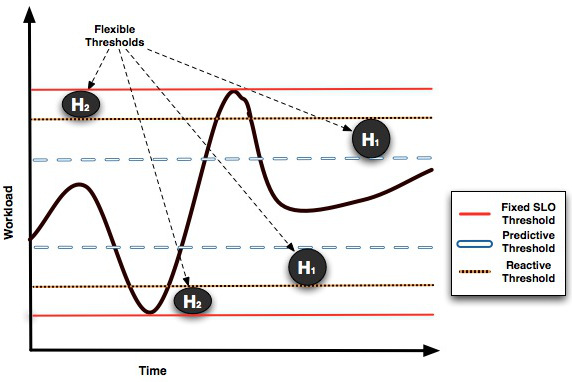
\includegraphics[width=7cm, height=5.3cm]{./images/thresholdGraphic.jpg}
\end{center}
\caption{Flexible thresholds}
\label{flexibleThresholds}
\end{figure}

\textbf{Workload's trend estimation:} Nowadays, there is a wide literature on mathematical models that try to predict future alterations in web application's workload. However, the workload mix and network traffic of web applications make more difficult to provide accurate predictions using these models. Besides, the complexity of these models sometimes prevent its integration into real auto scaling systems. To design a robust and simple provisioning system, we decided to use a feedback mechanism that analyzes the behavior of the system performance during an interval of time. An exhaustive analysis of the monitoring data during a small interval of time (approx. during the last 30min) provides enough information to detect the workload's trend, and thereby to classify the type of workload alteration as \emph{constant} or \emph{temporal}. Obviously, only \emph{constant} variations may trigger scaling actions to avoid frequent fluctuations in the system performance caused by short and sudden \emph{temporal} variations (flash crowds), as we will detail in Section~\ref{experiments}. Note that, the workload trend estimation is not the trigger of this algorithm, but one more mechanism in it. So, it could be also calculated by using mathematical model such linear regression, kernel canonical correlation, and so on.

%In order to take scaling decisiong using the weighted-metric feedback algorithm we now collect application-specific metrics for our measurements, evaluate the %evolution of the application workload avoiding an excessive reactive behavior, and handle threshold values that helps to predict possible SLA violations. 

%In particular, the profiling techniques appears as a solution to tackle this problems of heterogeneity.
\vspace{3mm}

Anyway, the use of these three mechanisms must follow an order when making scaling decisions, as illustrated in Algorithm~\ref{history_prov}. Initially, the user has to specify the thresholds ranges and give a weight to each metric. Next the flexible thresholds are defined based on Amazon recommendations and statistically-chose performance measures~\footnote{These performance values are obtained from previous executions of the same application using similar hardware configurations.}. Once the monitoring data is collected from the agents, the decision making process can start. Firstly, these data is analyzed to verify if it exceeds the predictive threshold ranges (denoted by \emph{p\_thr}), if so the probability of triggering scaling actions increases proportionally in function of the metric's weight. In order to keep track of workload variations, this algorithm stores in a queue (denoted by \emph{q}) the most recent system performance values, and analyzed them  to estimate the workload trend (denoted by \emph{td}). Finally, to trigger any scaling action, a serie of conditions have to be satisfied: (i) no previous scaling actions have been taken over the last 15min; (ii) the recent monitoring data have to exceed the reactive threshold ranges; (iii) the workload trend has to follow a constant pattern (increasing/decreasing); and (iv) the result of predictive thresholds evaluation has to match up with that obtained in (ii). 

\subsubsection{Problematic of this algorithm}

Although the combination of these techniques improves the accuracy of our measurements, and avoids to present an excessive reactive behavior. The heterogeneous nature of the VM instances and the workload require more flexible provisioning algorithms, as we pointed out in ~\cite{jiangThesis}. . 

\subsection{Workload mix-aware provisioning}


%The heterogeneity of cloud platforms, and therefore, of their VMs affect to the accuracy of the provisioning decisions. VMs with better hardware configuration can sustain higher workload intensities. In addition, the mixture of static/dynamic requests included into the workload of web applications makes more difficult to distribute these requests across multiple backend servers. Most of existing web load-balancer systems provide simple methods which do not consider the workload mix. Hence, methods such as\emph{round-robin} distributes the requests according to the servers with respect of its server weight; and the \emph{least connections} method which distributes requests to the server with the least connections. Unfortunately, these load-distribution methods are not so accurate when having a large diversity in the complexity of the requests. 

%As a solution, the workload mix-aware algorithm proposes to use a dynamic-weight load balancing method in conjunction with the weighted-metric feedback algorithm. By using this dynamic load-balancing mechanism, each backend server has a weight value which is dynamically adjusted based on its monitoring data, and thereby based on its own performance behavior. This mechanism allows to distribute requests across the servers taken into consideration the current workload intensity and the server throughput, which vary depending of its hardware configuration. As illustrated in Algorithm~\ref{mix_prov}, this algorithm assigns the same weight to each backend servers at the beginning of the process, and progressively adjusts their weights  (every $\sim$ 15min) depending on the monitoring data collected from each backend. By doing so, the load-balancing takes into account the complexity of the served requests and inherently the server throughput improving the distribution.

Another problem that we need to consider is the heterogeneity of cloud platforms.
Different virtual machines from the same cloud might have different performance
characteristics, even when their specifications from the cloud vendor are the same.
This problem can be addressed through various load balancing techniques, like
assigning weights to the backend servers or taking into account the current number
of connections that each server handles. Furthermore, the performance behavior
of the virtual servers can also change in time, either due to changes in
the application's usage patterns, or due to changes related to the hosting
of the virtual servers (e.g., VM migration).

In order to address these issues in ConPaaS we implemented a weighted load balancing
system in which the weights of the servers are periodically re-adjusted
automatically, based on the monitoring data. As illustrated in 
Algorithm~\ref{mix_prov}, this method assigns the same weight to each 
backend server at the beginning of the process. The weights are then periodically
adjusted (every $\sim$ 15min) depending on the average response time
of each server during this time interval.


\begin{algorithm}
{\scriptsize
\SetAlgoLined
\SetInd{0mm}{2mm}
\KwData{\\
\hspace{3mm} System and App-level metrics\\
\hspace{6mm} - Pre-defined metric threshold ranges, \emph{threshold}\\
\hspace{3mm} Define the weight of each metric, \emph{w}
}
\KwResult{Scaling decisions}
\BlankLine
Create a queue to store historical workload, \emph{q}\;
Establish flexible thresholds from \emph{threshold} ranges\;
\hspace{3mm}	- Scalings operations could be triggered, \emph{pred\_thr}\;
\hspace{3mm}	- Scalings operations must be triggered, \emph{reac\_thr}\; 
Initialize load-balancing weights for the backend servers\;
\BlankLine
\While{auto-scaling is ON}{
Collect monitoring data of each metric, \emph{data}\;

\uIf{ data$_i$ $>=$ pred\_thr$_i$}{
	Increment chances of \emph{scaling\_out} using \emph{w$_i$}, \emph{s\_out}\;
}\ElseIf{ data$_i$ $<$ pred\_thr$_i$}{
	Increment chances of \emph{scaling\_in} using $w_i$, \emph{s\_in}\;
}
\BlankLine
Add to \emph{q} the most recent workload value\;
Estimate historical workload trends (last $\sim$20min), \emph{td}\;
\hspace{3mm}	- If trend is increasing then \emph{td} = 1\;
\hspace{3mm}	- If trend is decreasing then \emph{td} = 0\;		
\BlankLine
\While{ no recent scaling operation}{
\uIf{ data$_i$ $>=$ reac\_thr$_i$ \textbf{and}  $td$ = 1 \textbf{and} \emph{s\_out} $>=$ \emph{s\_in}}{
	ADD resources\;
}
\ElseIf{ data$_i$ $<$ reac\_thr$_i$ \textbf{and} \emph{td} = 0 \textbf{and} s\_out $<$ s\_in }{
	REMOVE resources\;
}
}
\BlankLine
Adjust load-balancing weights based on the workload ($\sim$15min)\;
}
}
\caption{Workload mix-aware}
\label{mix_prov}
\end{algorithm}


%\fixme{unlike in some synthetic benchmarks, in Wikipedia there are large variations
%in the complexity of the articles; so the PHP processing time is more difficult 
% to predict}

%\begin{figure}
%\begin{center}
%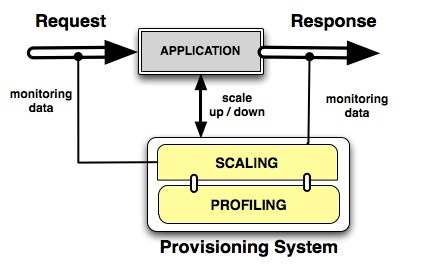
\includegraphics[width=0.4\textwidth, height=4cm]{./images/monitoringSchema.jpg}
%\end{center}
%\label{model}
%\caption{Profiling Resource Provisioning}
%\end{figure}
